%% This is an example first chapter.  You should put chapter/appendix that you
%% write into a separate file, and add a line \include{yourfilename} to
%% main.tex, where `yourfilename.tex' is the name of the chapter/appendix file.
%% You can process specific files by typing their names in at the 
%% \files=
%% prompt when you run the file main.tex through LaTeX.

\chapter{Arquitectura Propuesta}

\section{Formato del artículo}

El texto mostrado en la figura \ref{formato} esta formado por secciones encerradas entre llaves que pueden contener  bloques de texto. Los bloques de texto pueden ser de longitud arbitraria, puede abarcar desde una palabra hasta varios párrafos. Estos bloques de texto están divididos por barras, los bloques de texto que se encuentren fuera de los paréntesis (representados en color negro en la figura \ref{formato}) no tendrán ninguna alteración al evolucionar los textos.

\begin{figure}[htp]
  \centerline{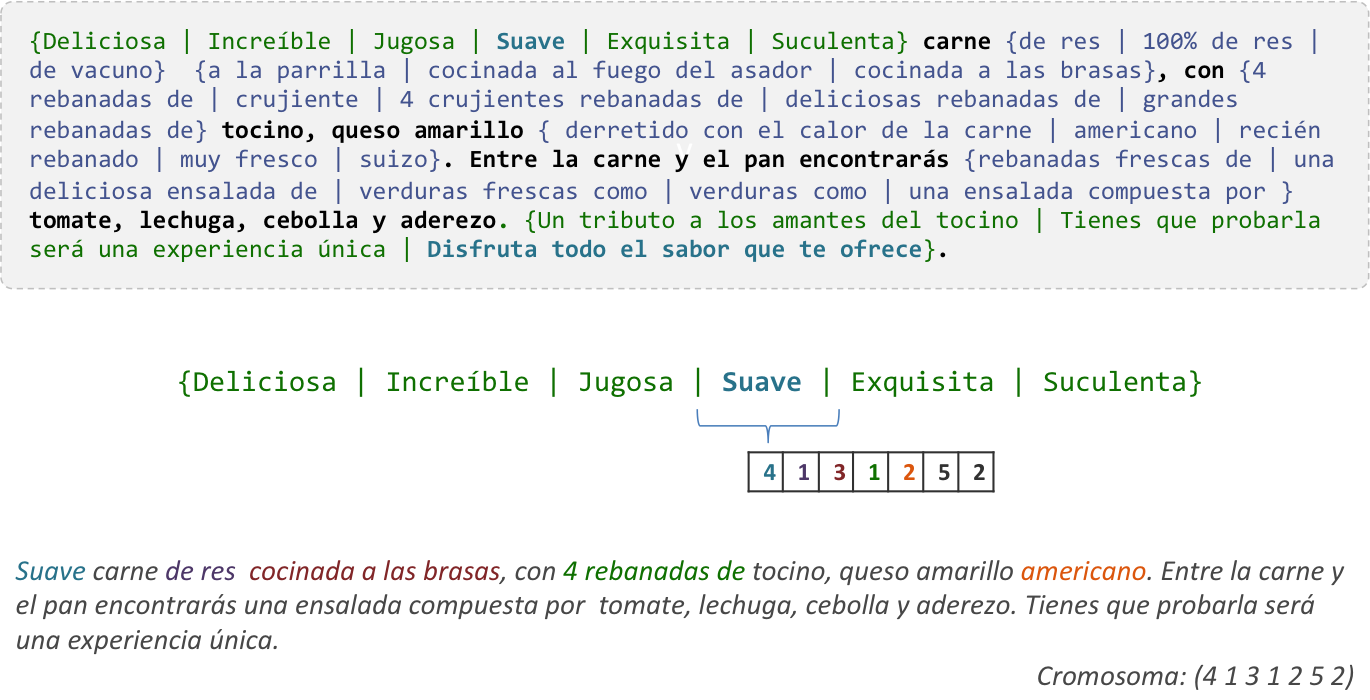
\includegraphics[width=6in]{formato.png}} 
  \caption{Formato del texto} 
\label{formato}
\end{figure}


El texto esta representado por un vector donde cada número indica la posición del bloque de texto al que se refiere, si la palabra que se quiere representar en la figura \ref{formato} es "Suave" entonces el vector indicará con el número 4 que la palabra se encuentra en la cuarta posición dentro de las opciones que el autor sugirió.


\clearpage
\section{Optimizacion del texto}

Se determinarán las mejores combinaciones utilizando un algoritmo genético, los pasos para evolucionar los textos generando nuevos individuos con mejores caracteristicas segun las elecciones de los usuarios son los siguientes.

\begin{enumerate}[\hspace*{0.5cm} P{a}so 1]
\item Se genera una población aleatoria de 100 individuos.
\item Se seleccionan 12 cromosomas, 6 del padre y 6 de la madre como se muestra en la figura \ref{padres}.

\begin{figure}[htp]
  \centerline{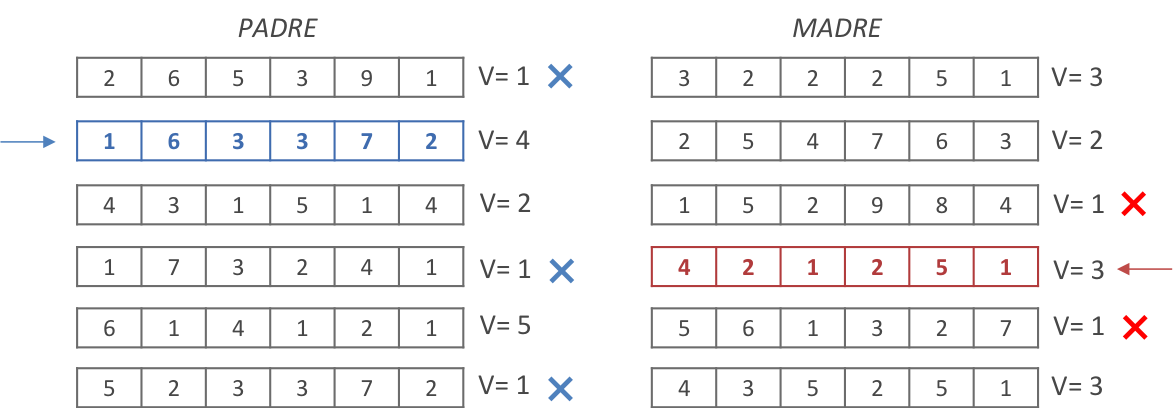
\includegraphics[width=6in]{padres.png}} 
  \caption{Seleccion de los cromosomas padres} 
\label{padres}
\end{figure}

\item Se calcula el fitness para seleccionar a los padres con mayor puntuación. La ecuación para calcular el ftiness es la siguiente:

\begin{equation}
Fitness = \frac{s+1 }{v+1 }   \textup{ donde }   \begin{matrix} \textup{ s = seleccion del texto} \\ \textup{ v = vistas del texto}\end{matrix}
\end{equation}

\item Se selecciona aleatoriamente  el tipo de cruce (los tipos de cruce se muestran en la figura \ref{cruce} ). La probabilidad de selección de alguno de los dos tipos de cruce es igual para ambos.

\begin{figure}[htp]
  \centerline{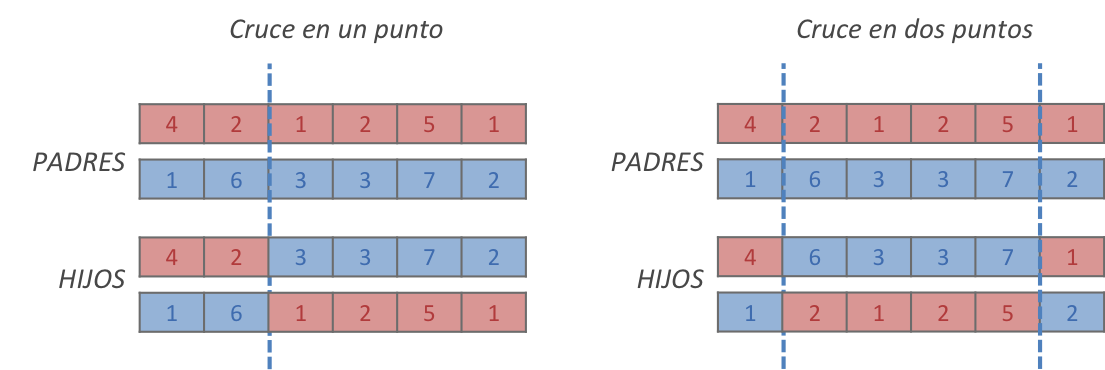
\includegraphics[width=6in]{cruce.png}} 
  \caption{Tipos de cruce utilizados} 
\label{cruce}
\end{figure}

\item Se crean dos nuevos cromosomas hijos. Hay una probabilidad del 10\% de que se efectúe una mutación para ambos cromosomas.
\item Se eliminan de la muestra los 2 cromosomas (un padre y una madre) con fitness más bajo y los hijos toman su lugar.
\end{enumerate}



